\section{tasks::plotorders Class Reference}
\label{classtasks_1_1plotorders}\index{tasks::plotorders@{tasks::plotorders}}
Inheritance diagram for tasks::plotorders::\begin{figure}[H]
\begin{center}
\leavevmode
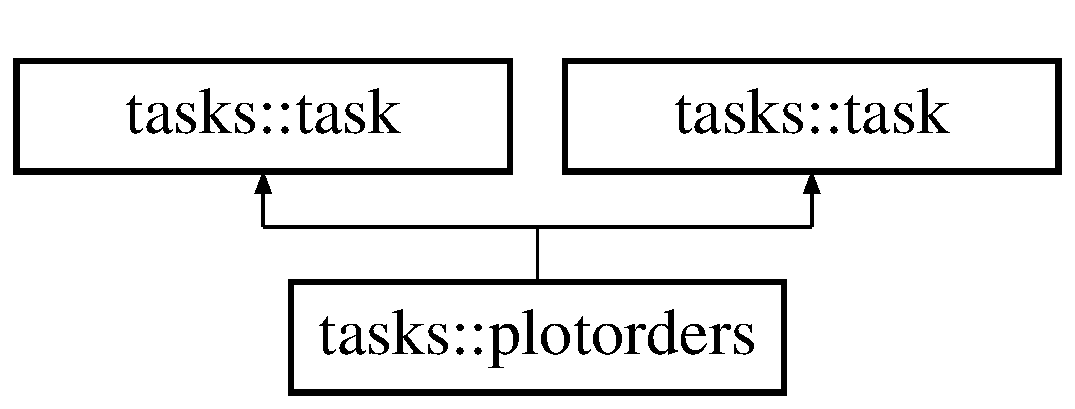
\includegraphics[height=2cm]{classtasks_1_1plotorders}
\end{center}
\end{figure}
\subsection*{Public Member Functions}
\begin{CompactItemize}
\item 
def \textbf{run}\label{classtasks_1_1plotorders_ecce56a8e01f10a140447e4d72ee0345}

\item 
def \textbf{run}\label{classtasks_1_1plotorders_ecce56a8e01f10a140447e4d72ee0345}

\end{CompactItemize}
\subsection*{Static Public Attributes}
\begin{CompactItemize}
\item 
string \textbf{name} = '{\bfplotorders}'\label{classtasks_1_1plotorders_0c6084994b35b41a52c644a4c210711d}

\item 
string \textbf{button\-Text} = 'Plot order locations'\label{classtasks_1_1plotorders_cfa6bb99516329101ddf983993a72031}

\end{CompactItemize}


\subsection{Detailed Description}


\footnotesize\begin{verbatim}Show (schematically) the recovered location of the spectral orders.
\end{verbatim}
\normalsize
 



The documentation for this class was generated from the following files:\begin{CompactItemize}
\item 
old/PANICtool-1.0/tasks.py\item 
old/tasks.py\end{CompactItemize}
